

\begin{figure}[!h]
\centering
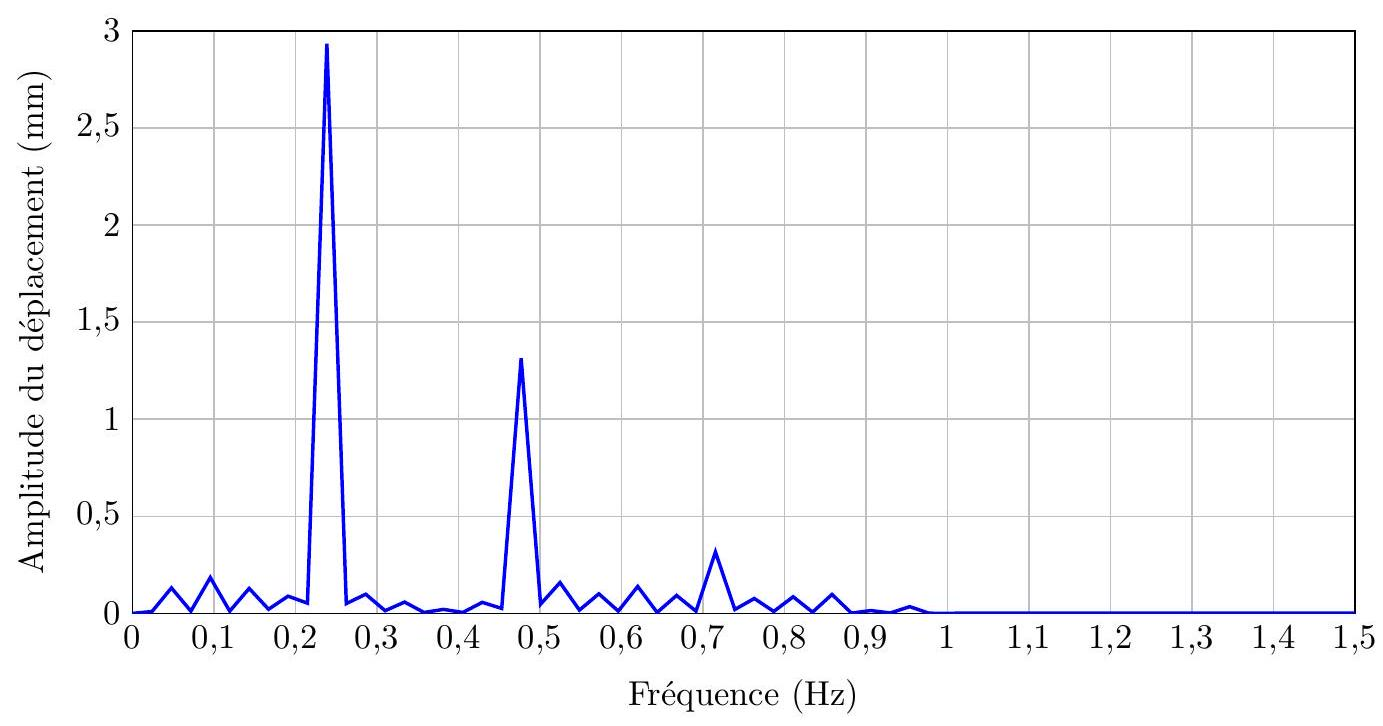
\includegraphics[max width=\textwidth]{2024_08_29_b4f920ed3822451bf72bg-05}
%Figure 5 
\caption{\label{fig_05} Contenu spectral du déplacement dû aux mouvements physiologiques}
\end{figure}


% I.B - 
\section{Cahier des charges partiel de la chaine d'asservissement en position du robot esclave}
%\section{Objectif}
\begin{obj}
Déterminer une valeur numérique pour la bande passante de l'asservissement en position du robot esclave et vérifier le cahier des charges associé.
\end{obj}

Pour cette partie, on retient le modèle de signal de déplacement idéal $z^{*}(t)$ défini précédemment. L'objectif de cette partie est de déterminer la bande passante minimale $\omega_{0 \text { min }}$ en boucle fermée de la chaine d'asservissement permettant d'assurer la précision demandée par le diagramme des exigences.\\
Pour cette pré-détermination, on utilise un modèle simple en raisonnant sur un mouvement selon un seul axe assuré par une chaine d'asservissement (non représentée) dont on note $F(p)$ la fonction de transfert en boucle fermée telle que $F(p)=\frac{Z(p)}{Z^{*}(p)}=\frac{\omega_{0}^{2}}{p^{2}+2 \xi \omega_{0} p+\omega_{0}^{2}}$ où $z^{*}(t)$ est la consigne de déplacement (en mm) et $z(t)$ la sortie de la chaine d'asservissement (en mm). Vis-à-vis de ce signal de consigne, on note l'écart

$$
\varepsilon(t)=z^{*}(t)-z(t)=\varepsilon_{2} \sin \left(2 \pi f_{2} t+\Theta_{2}\right)=\varepsilon_{2} \sin \left(\omega_{2} t+\Theta_{2}\right)
$$

%Q 7. 
\question{On note $H(p)=\frac{\varepsilon(p)}{Z^{*}(p)}$ la fonction de transfert de la consigne $Z^{*}(p)$ vers l'écart $\varepsilon(p)$. Déterminer $H(p)$ en fonction de $\omega_{0}$ et $\xi$. Donner les relations exprimant $\varepsilon_{2}$ et $\Theta_{2}$ en fonction de $\left\|H\left(\mathrm{i} \omega_{2}\right)\right\|$, $\arg \left(H\left(\mathrm{i} \omega_{2}\right)\right), A_{2}$ et $\Phi_{2}$.}

% Q 8. 
\question{En considérant la bande de pulsations $\omega \ll \omega_{0}$, donner une approximation de $\|H(\mathrm{i} \omega)\|$ sous la forme $\|H(\mathrm{i} \omega)\| \approx K \omega$ où $K$ est un gain à préciser. En considérant cette approximation, donner alors une expression de $\varepsilon_{2}$ en fonction de $A_{2}, \omega_{2}, \omega_{0}$ et $\xi$.}

%Q 9. 
\question{En considérant $\varepsilon_{2}$, déterminer la valeur minimale de $\omega_{0}$ permettant d'assurer la précision exigée vis-àvis de la consigne sinusoïdale de pulsation $\omega_{2}=2 \pi f_{2}$ (pour l'application numérique, on adoptera un coefficient d'amortissement $\xi=1$ ). Vérifier si l'application numérique est compatible avec celle exprimée par le diagramme des exigences (figure \ref{fig_03} et plus précisément l'exigence 1.2.3).}

Dans la suite du sujet, il s'agit de déterminer une loi de commande de la chaine d'asservissement permettant d'assurer les exigences du cahier des charges. Cette loi de commande devra résoudre le problème mis en évidence et assurer la compatibilité entre la bande passante minimale et le niveau de précision requis vis-à-vis des consignes sinusoïdales. La conception de cette loi de commande nécessite au préalable de définir et identifier un modèle dynamique du robot esclave, c'est l'objet de la partie suivante.

\section{Analyse géométrique et élaboration du modèle dynamique du robot esclave}
%\section{Objectif}
\begin{obj}
Vérifier la capabilité du robot esclave à respecter le cahier des charges et déterminer le modèle dynamique d'un des axes du robot esclave utilisé pour dimensionner sa commande.
\end{obj}

Ce robot, dont une photo est donnée en figure \ref{fig_06}, est constitué de bras motorisés adaptés à la chirurgie miniinvasive et dispose de quatre mouvements actionnés par des moteurs électriques, dont trois sont visibles sur la figure \ref{fig_06} .

\begin{figure}[!h]
\centering
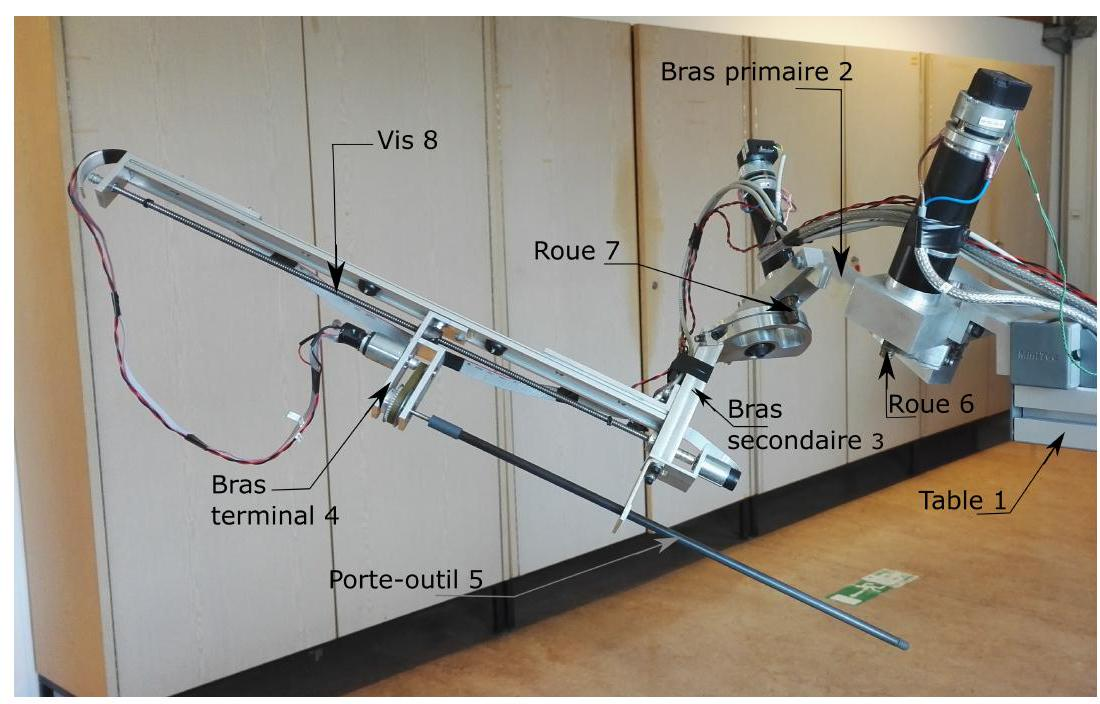
\includegraphics[max width=\textwidth]{2024_08_29_b4f920ed3822451bf72bg-06}
\caption{\label{fig_06}Robot esclave}
\end{figure}

Le schéma cinématique donné en figure \ref{fig_07} est une représentation de la modélisation retenue pour une configuration particulière du robot dans laquelle tous les bras sont coplanaires. Pour ce modèle, le robot est constitué :

\begin{itemize}
  \item d'une table 1 , considérée comme fixe à laquelle on associe un référentiel galiléen $\left(O, \vec{x}_{0}, \vec{y}_{0}, \vec{z}_{0}\right)$, dont $\vec{z}_{0}$ est la verticale ascendante, et un repère $\left(A, \vec{x}_{0}, \vec{y}_{1}, \vec{z}_{1}\right)$, avec $\alpha_{1}=\left(\vec{y}_{0}, \vec{y}_{1}\right)=\left(\vec{z}_{0}, \vec{z}_{1}\right)=\pi / 4 \mathrm{rad}$ et $\overrightarrow{O A}=l_{0} \vec{y}_{0}+l_{1} \vec{y}_{1}$;
  \item d'un bras primaire 2, en liaison pivot d'axe $\left(A, \vec{z}_{1}\right)$ avec la table 1 , auquel on associe un repère $\left(A, \vec{x}_{2}, \vec{y}_{2}, \vec{z}_{1}\right)$, avec $\theta_{21}=\left(\vec{x}_{1}, \vec{x}_{2}\right)=\left(\vec{y}_{1}, \vec{y}_{2}\right)$, et un second repère $\left(B, \vec{x}_{2}{ }^{\prime}, \vec{y}_{2}{ }^{\prime}, \vec{z}_{2}{ }^{\prime}\right)$, avec $\alpha_{2}=\left(\vec{y}_{2}, \vec{y}_{2}{ }^{\prime}\right)=\left(\vec{z}_{1}, \vec{z}_{2}{ }^{\prime}\right)=-\pi / 4 \mathrm{rad}$ et de plus $\overrightarrow{A B}=l_{2} \vec{y}_{2}+l_{2}^{\prime} \vec{y}_{2}{ }^{\prime}$, avec $l_{2}=0,3 \mathrm{~m}$ et $l_{2}^{\prime}=0,44 \mathrm{~m}$;
  \item d'un bras secondaire 3, en liaison pivot d'axe $\left(B, \vec{z}_{2}{ }^{\prime}\right)$ avec le bras primaire 2 , auquel on associe un repère $\left(B, \vec{x}_{3}, \vec{y}_{3}, \vec{z}_{3}\right)$, avec $\theta_{32}=\left(\vec{x}_{2}{ }^{\prime}, \vec{x}_{3}\right)=\left(\vec{y}_{2}{ }^{\prime}, \vec{y}_{3}\right)$
  \item d'un bras terminal 4 , en liaison glissière de direction $\vec{z}_{3}$ avec le bras secondaire 3 . On note $\vec{B} C=l_{3} \vec{y}_{3}+\lambda(t) \vec{z}_{3}$, avec $l_{3}=0,92 \mathrm{~m} ;$
  \item d'un porte-outil 5 , en liaison pivot d'axe $\left(C, \vec{z}_{3}\right)$ avec le bras terminal 4. L'outil lié au porte-outil 5 est caractérisé par le point $D$, désignant le point actif de l'outil (point effectuant l'opération d'incision). On note $\overrightarrow{C D}=l_{4} \vec{z}_{4}$\\
La liaison pivot entre le porte-outil 5 et le bras terminal 4 permet d'obtenir une rotation de l'outil utilisé autour de son axe principal. Elle ne sera pas utilisée dans cette étude, le porte-outil 5 est supposé être immobile par rapport au bras 4 .\\
Les autres mouvements sont générés par des ensembles motoréducteurs:
  \item un premier motoréducteur entraine la roue dentée 6 , qui elle-même entraine une seconde roue dentée liée au bras primaire 2. L'action du motoréducteur sur la roue dentée 6 est modélisée par un couple dont le moment est noté $\vec{C}_{m 1}=C_{m 1} \vec{z}_{1}$
  \item un second motoréducteur entraine l'arbre 7 sur lequel est installé le pignon d'attaque du réducteur 9 . Ce pignon entraine une roue dentée liée au bras secondaire 3 . Le rapport de transmission de ce réducteur 9 est noté $r_{9}$ avec $r_{9}=\frac{\dot{\theta}_{32}}{\dot{\theta}_{72}}=0,25$. Son rendement est noté $\eta_{9}$ avec $\eta_{9}=0,78$. L'action du motoréducteur sur l'arbre 7 est modélisée par un couple dont le moment est noté $\vec{C}_{m 2}=C_{m 2} \vec{z}_{2}{ }^{\prime}$;
  \item enfin, le troisième motoréducteur entraine la vis 8 d'un système vis-écrou dont l'écrou est lié au bras terminal 4. Cette vis est de pas à droite $p=0,63 \mathrm{~mm}$. L'angle de rotation de la vis 8 par rapport au bras secondaire 3 est noté $\theta_{83}$ avec $\theta_{83}=\left(\vec{x}_{3}, \vec{x}_{8}\right)$. L'action du motoréducteur sur la vis 8 est modélisée par un couple dont le moment est noté $\vec{C}_{m 3}=C_{m 3} \vec{z}_{3}$.
\end{itemize}


\begin{figure}[!h]
\centering
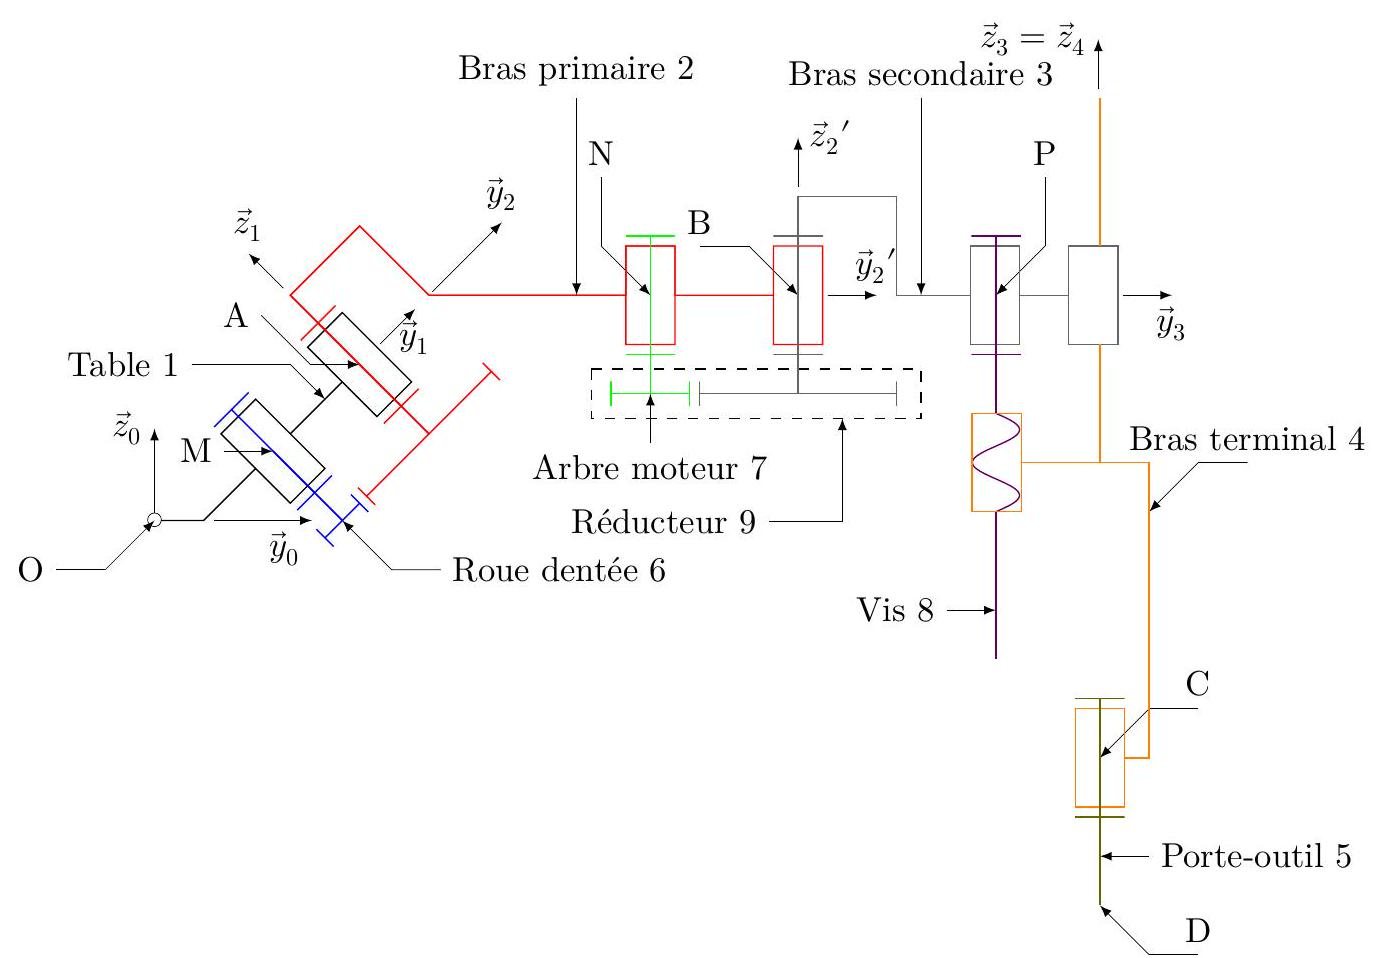
\includegraphics[max width=\textwidth]{2024_08_29_b4f920ed3822451bf72bg-07(1)}
\caption{\label{fig_07} Schéma cinématique 2 D du robot esclave}
\end{figure}

On donne de plus, les caractéristiques suivantes.

\begin{itemize}
  \item Pour le bras secondaire 3
  \item $G_{3}$ son centre de gravité (non représenté sur la figure \ref{fig_07}), défini par $\overrightarrow{B G_{3}}=a_{3} \vec{y}_{3}+b_{3} \vec{z}_{3}$, avec $a_{3}=0,22 \mathrm{~m}$ et $b_{3}=0,15 \mathrm{~m}$;
  \item $J_{3}=6 \times 10^{-1} \mathrm{~kg} \cdot \mathrm{m}^{2}$, son moment d'inertie autour de l'axe $\left(B, \vec{z}_{3}\right)$;
  \item $m_{3}=35,2 \mathrm{~kg}$, sa masse.
  \item Pour le bras terminal 4
  \item $G_{4}$ son centre de gravité (non représenté sur la figure \ref{fig_07}), défini par $\overrightarrow{C G_{4}}=b_{4} \vec{z}_{4}$, avec $b_{4}=0,36 \mathrm{~m}$;
  \item $J_{4}=2,2 \times 10^{-1} \mathrm{~kg} \cdot \mathrm{m}^{2}$, son moment d'inertie autour de l'axe $\left(G_{4}, \vec{z}_{4}\right)$;
  \item $m_{4}=18,4 \mathrm{~kg}$, sa masse.
  \item Les caractéristiques de masse et d'inertie des autres ensembles seront négligées devant celles du bras secondaire 3 et de l'arbre terminal 4 .\\
Le paramétrage angulaire du mécanisme est représenté figure \ref{fig_08}.
\end{itemize}


\begin{figure}[!h]
\centering
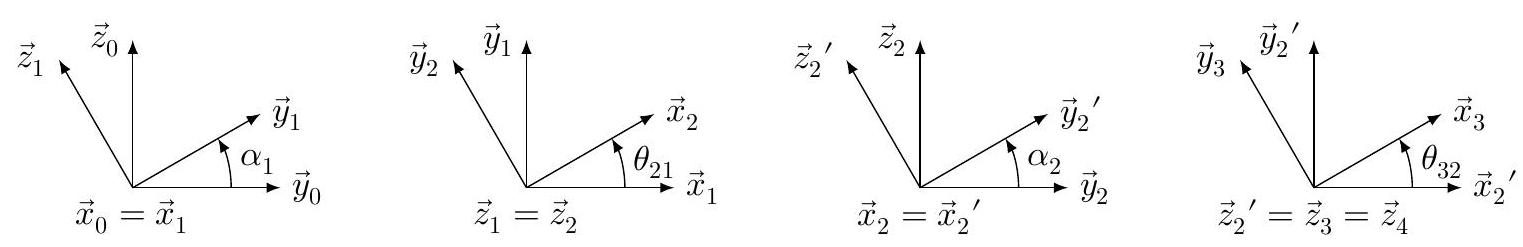
\includegraphics[max width=\textwidth, center]{2024_08_29_b4f920ed3822451bf72bg-07}
\caption{\label{fig_08} Paramétrage angulaire utilisé}
\end{figure}

Afin de déterminer la loi de commande des différents actionneurs, il est nécessaire de connaitre l'influence des différentes actions mécaniques sur le système. On prendra pour la suite de l'étude l'hypothèse que, hormis les liaisons internes au réducteur 9 entre l'arbre moteur 7 et le bras secondaire, les liaisons seront considérées comme parfaites. De plus, on étudiera le robot esclave dans une configuration et pour une commande particulières. En effet, le comportement du système lors de sa phase d'approche de l'organe à opérer est bien moins « sensible » que celui aux alentours de l'organe et lors d'une incision. Ainsi on considérera un mouvement particulier de l'outil chirurgical correspondant à une configuration du robot pré-établie en amont de l'opération. Dans ce cas, on suppose que :

\begin{itemize}
  \item le mouvement relatif entre le bras primaire 2 et la table 1 est nul avec $\dot{\theta}_{21}=0$ et $\theta_{21}=\pi / 3 \mathrm{rad}$. Le point $B$ est alors immobile dans $\left(O, \vec{x}_{0}, \vec{y}_{0}, \vec{z}_{0}\right)$;
  \item à partir d'une position initiale $(t=0)$ de $3 / 2$ telle que $\theta_{32}(t=0)=0$, le mouvement de $3 / 2$ reste de faible amplitude avec $\lambda(t=0)=\lambda_{0}=-0,80 \mathrm{~m}$ et $\theta_{83}(t=0)=0$
  \item le mouvement entre le porte outil 5 et le bras terminal 4 est nul ;
  \item l'action de l'organe opéré sur le porte-outil est négligée devant les autres actions mises en jeu.
\end{itemize}

%II.A - 
\subsection{Vérification de la capabilité du robot esclave}
\begin{obj}
Vérifier la capacité du robot esclave à respecter l'exigence de précision 1.3.3 et dimensionner les capteurs installés sur le robot en conséquence.
\end{obj}

Afin de pouvoir asservir en position le robot esclave, il est nécessaire que la mesure de la position de l'outil soit la plus précise possible. En ce sens, il est nécessaire que la résolution de cette mesure (la plus petite valeur de déplacement mesurable) soit, dans le pire des cas, égale à l'écart maximal autorisé par le cahier des charges.\\
On étudiera uniquement l'influence du robot esclave sur l'écart de position de l'outil. Ainsi, cet écart ne dépend que de la structure cinématique du robot esclave et des capteurs utilisés pour l'asservissement. On considère pour la suite que si le robot esclave est capable de compenser les signaux physiologiques présentés figure \ref{fig_04} en respectant l'exigence 1.3.3 du cahier des charges présenté figure \ref{fig_03}, il sera aussi capable de respecter ce cahier des charges pour la consigne donnée par le chirurgien à l'aide du robot maitre.\\

%Q 10. 
\question{À partir de la figure \ref{fig_04}, déterminer la valeur numérique de $s_{\text {max }}$, la résolution maximale de mesure sur la position de l'outil lors d'une opération pour respecter l'exigence 1.3.3 du cahier des charges présenté figure \ref{fig_03}. La mise en place pré-opératoire définie précédemment permet de considérer que le repère $\left(B, \vec{x}_{2}{ }^{\prime}, \vec{y}_{2}{ }^{\prime}, \vec{z}_{2}{ }^{\prime}\right)$ est un référentiel galiléen. C'est à partir de ce repère que sont définies les trajectoires de l'outil lors de l'opération.}

%Q 11. 
\question{En traduisant la propriété cinématique de la liaison hélicoïdale de pas à droite $p$ et d'axe $\left(P, \vec{z}_{3}\right)$ entre les solides 4 et 8 , donner la relation liant $\lambda(t), \lambda_{0}, p$ et $\theta_{83}$. En déduire l'expression du vecteur position $\overrightarrow{B D}$ caractérisant le point opératoire de l'outil dans la base $\left(\vec{x}_{3}, \vec{y}_{3}, \vec{z}_{3}\right)$ en fonction de $l_{3}, l_{4}, \lambda_{0}, p$ et $\theta_{83}(t)$.}

%Q 12. 
\question{En supposant que $\theta_{32}(t)$ reste de faible amplitude, exprimer les coordonnées $\left(x_{D}, y_{D}, z_{D}\right)$ du vecteur $\overrightarrow{B D}$ dans la base $\left(\vec{x}_{2}{ }^{\prime}, \vec{y}_{2}{ }^{\prime}, \vec{z}_{2}{ }^{\prime}\right)$ en fonction $l_{3}, l_{4}, \lambda_{0}, p, \theta_{32}(t)$ et $\theta_{83}(t)$.}

Afin de déterminer la résolution de mesure $s_{D}$ sur le déplacement du point $D$, il est choisi d'utiliser une hypothèse de propagation quadratique des incertitudes avec un coefficient de sécurité de 3 . Ainsi, on peut écrire

$$
s_{D}=3 \sqrt{s_{X}^{2}+s_{Y}^{2}+s_{Z}^{2}}
$$

où $s_{X}, s_{Y}$ et $s_{Z}$ sont les résolutions de mesure respectivement suivant les directions $\vec{x}_{2}{ }^{\prime}, \vec{y}_{2}{ }^{\prime}$ et $\vec{z}_{2}{ }^{\prime}$.\\
Afin de réaliser l'asservissement du robot esclave, deux capteurs identiques permettant la mesure des angles $\theta_{32}$ et $\theta_{83}$ ont été mis en œuvre. On note la résolution de ces capteurs $s_{\text {capteur }}$.\\

%Q 13. 
\question{Exprimer $s_{D}$ en fonction de $l_{3}$, $p$, et la résolution de mesure sur les angles $s_{\text {capteur }}$. En déduire la valeur maximale de $s_{\text {capteur }}$ pour pouvoir respecter l'exigence 1.3.3 du cahier des charges.}

%II.B - 
\subsection{Détermination et vérification du modèle dynamique du robot esclave}
\begin{obj}
Déterminer le modèle dynamique du robot esclave en vue de l'élaboration de sa commande.
\end{obj}
%II.B.1)
\subsubsection{Vérification du fonctionnement du réducteur 9}
Le réducteur 9 , monté entre l'arbre moteur 7 et le bras secondaire 3 , représenté sur la figure \ref{fig_07} par un ensemble de deux roues dentées est en fait un train épicycloïdal. L'action de l'arbre de sortie de ce réducteur sur le bras secondaire est modélisée par un couple dont le moment est noté $\vec{C}_{73}=C_{73} \vec{z}_{2}{ }^{\prime}$.

On se propose de vérifier les caractéristiques du réducteur fournies par le constructeur (rendement et rapport de transmission) dans l'optique de l'élaboration du modèle dynamique du robot.

%Q 14. 
\question{Exprimer $\vec{C}_{73}$, le moment de l'action mécanique exercée par l'arbre moteur 7 sur le bras secondaire 3 en B, en fonction de $C_{m 2}, r_{9}$ et $\eta_{9}$.}

Un essai sur le réducteur 9 a permis d'obtenir la courbe figure \ref{fig_09} représentant l'évolution du couple en sortie du réducteur $C_{73}$ en fonction du couple en entrée $C_{m 2}$.\\
%Q 15. 
\question{Conclure sur la validité des valeurs de $r_{9}$ et $\eta_{9}$ fournies par le constructeur.}

% II.B.2) 
\subsubsection{Élaboration du modèle dynamique d'un axe du robot esclave}
Le graphe de structure de la modélisation retenue pour le système est donné sur la figure \ref{fig_A} du document réponse.\\
%Q 16. 
\question{Sur la figure \ref{fig_A}, donner le nombre d'inconnues d'actions mécaniques (noté NI-AM) pour chacune des liaisons représentées sur le graphe de structure et indiquer les actions extérieures auxquelles sont soumises les différentes classes d'équivalence cinématiques.}

%Q 17. 
\question{Proposer, le plus clairement et synthétiquement possible, sans calcul, une démarche qui permette d'exprimer le couple nécessaire $C_{m 2}$ à fournir sur l'arbre 7 du motoréducteur afin de réaliser le mouvement décrit précédemment.}


\begin{figure}[!h]
\centering
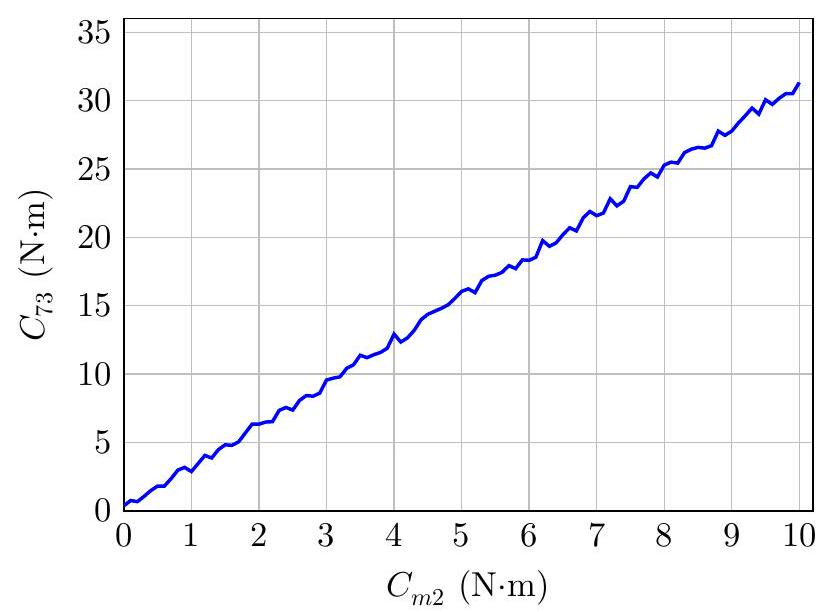
\includegraphics[max width=.7\textwidth]{2024_08_29_b4f920ed3822451bf72bg-09(1)}
\caption{\label{fig_09} Évolution de $C_{73}$ en fonction de $C_{m 2}$}
\end{figure}

%Q 18. 
\question{Exprimer $\vec{V}_{G_{4}, 4 / 1}$ la vitesse du point $G_{4}$ centre de gravité du bras terminal 4 dans son mouvement par rapport à la table 1 , en fonction de $l_{3}, \dot{\lambda}$ et $\dot{\theta}_{32}$.\\
Un essai a permis d'obtenir le relevé de mesure présenté figure \ref{fig_10} pour une loi de commande de $\theta_{32}(t)$ en trapèze de vitesse. On supposera que le temps de réponse du moteur est tel que l'évolution de la vitesse suit parfaitement son profil de commande.}


\begin{figure}[!h]
\centering
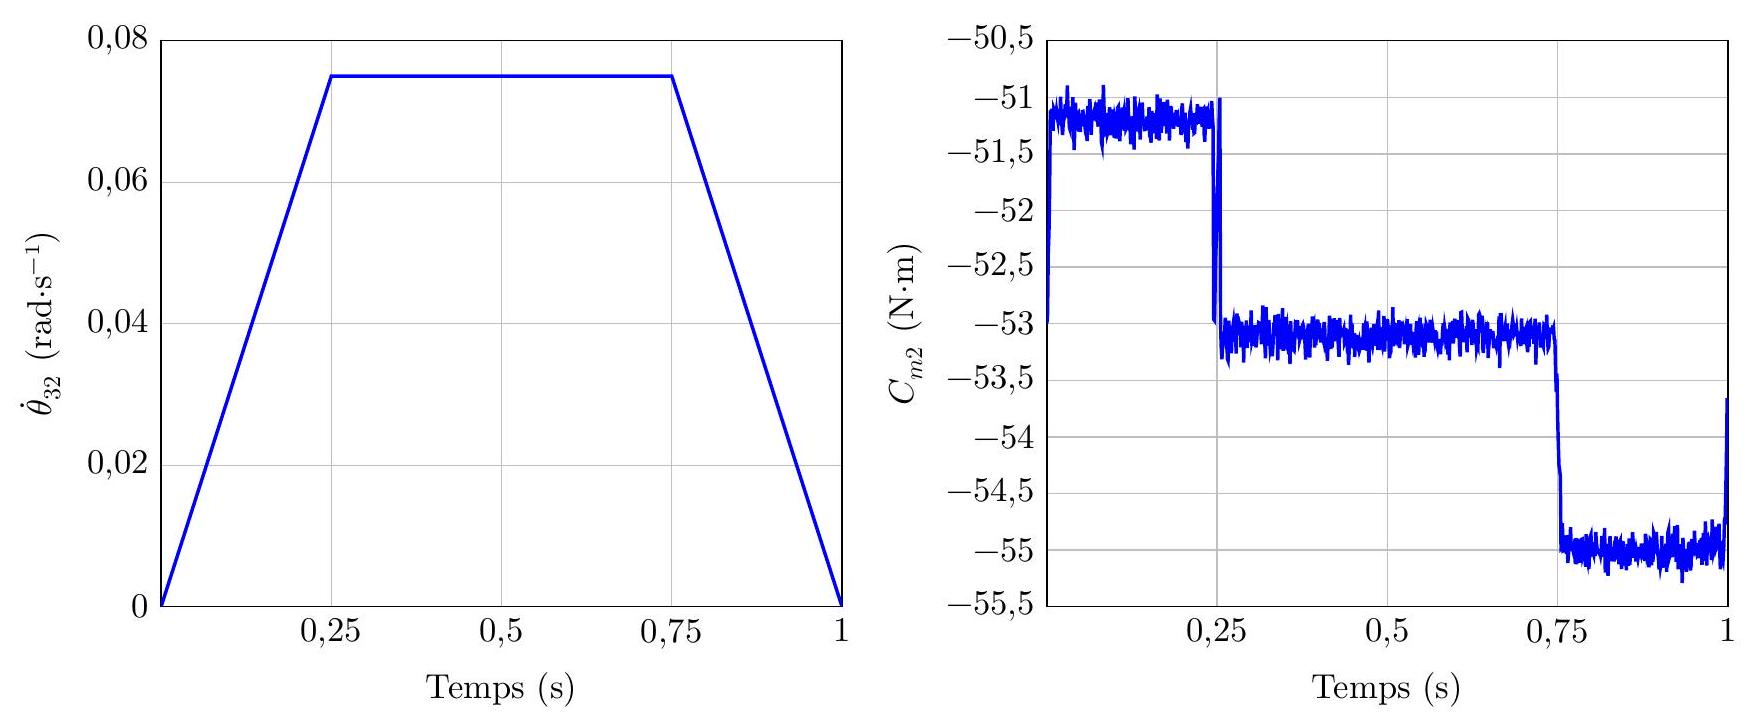
\includegraphics[max width=\textwidth]{2024_08_29_b4f920ed3822451bf72bg-09}
\caption{\label{fig_10} Évolution de $\dot{\theta}_{32}$ et de $C_{m 2}$}
\end{figure}

%Q 19. 
\question{Justifier l'hypothèse que la valeur de $\theta_{32}(t)$ reste faible. En déduire que l'on pourra considérer pour la suite que}
$$
\forall t, \quad \cos \left(\theta_{32}(t)\right) \approx 1 \quad \text { et } \quad \sin \left(\theta_{32}(t)\right) \approx 0
$$

%Q 20. 
\question{Exprimer $\vec{\delta}_{B, 4 / 1} \cdot \vec{z}_{4}$, la projection du moment dynamique au point $B$ appartenant au bras terminal 4 dans son mouvement par rapport à la table 1 sur la direction $\vec{z}_{4}$, en fonction de $J_{4}, m_{4}, l_{3}$ et $\ddot{\theta}_{32}$.\\}

%Q 21. 
\question{En appliquant le principe fondamental de la dynamique, exprimer le couple $C_{m 2}$ sous la forme}
$$
J_{e q} \ddot{\theta}_{32}(t)=A C_{m 2}(t)+C_{r}(t)
$$

Donner alors l'expression littérale, puis la valeur numérique de

\begin{itemize}
  \item $J_{e q}$ en fonction de $J_{3}, J_{4}, m_{4}$ et $l_{3}$;
  \item $A$ en fonction de $r_{9}$ et $\eta_{9}$
  \item $C_{r}(t)$ en fonction de $g$ (accélération de la pesanteur), $m_{3}, m_{4}, a_{3}, l_{3}, \alpha_{1}$ et $\theta_{21}$.
\end{itemize}

%Q 22.
\question{À partir de la figure \ref{fig_10}, déterminer les valeurs expérimentales du couple résistant $C_{r}(t)$ et de l'inertie équivalente $J_{\text {eq }}$ ramenée sur l'axe $\left(B, \vec{z}_{3}\right)$.}

%Q 23. 
\question{À partir de la figure \ref{fig_10}, en comparant les valeurs théoriques et expérimentales de l'inertie équivalente et du couple résistant ramenés sur l'arbre 7 du motoréducteur, expliquer les écarts éventuels et conclure sur la validité du modèle utilisé.}

\section{Définition et analyse de la chaine d'asservissement du robot esclave}
\begin{obj}
Définir le régulateur de la chaine d'asservissement du robot esclave, analyser ses performances vis-à-vis des perturbations en se limitant à celles dues aux couples de frottement sec et compléter la chaine d'asservissement par la compensation de ces efforts.
\end{obj}

Un robot étant un système multivariable comportant en particulier des couplages entre les dynamiques des différents axes, la mise en place d'une loi de commande prenant en compte tous les axes peut se révéler complexe. Dans le cadre de ce sujet, on suppose

\begin{itemize}
  \item que des boucles internes locales à chaque axe motorisé ont été mises en place pour asservir le couple de chaque articulation à un couple de référence. Ceci permet de considérer le robot comme un système dont les entrées sont les couples moteurs intervenant dans les différentes articulations ;
  \item que des termes de compensation active des couples dus à la pesanteur ont été mis en place sur chaque articulation ;
  \item que les couplages entre les axes sont modélisés comme des entrées de perturbation dans les chaines d'asservissement.\\
L'objectif de cette partie est de déterminer la loi de commande permettant d'assurer l'asservissement de position des articulations $\theta_{32}$ et $\theta_{21}$ à des angles de référence issus du modèle cinématique inverse (figure \ref{fig_02}). Pour la suite de l'étude, on note les positions articulaires $q_{j}=\theta_{j}[j=32,21]$ et les consignes pour les chaines d'asservissement associées $q_{j}^{*}=\theta_{j}^{*}[j=32,21]$.
\end{itemize}

\subsection{Calcul d'un correcteur et analyse partielle des performances de la chaine d'asservissement}
\begin{obj}
Déterminer un correcteur pour la chaine d'asservissement de la position angulaire des articulations. Afin d'aboutir à une démarche générale (indépendante d'une articulation particulière), la loi de commande sera paramétrée par le moment d'inertie équivalent de l'articulation considérée.
\end{obj}

Au regard des hypothèses précédentes, la synthèse du correcteur associé à une articulation $j$ peut être effectuée en utilisant le modèle suivant

$$
J_{e q} \ddot{q}_{j}(t)=c_{j}(t)+c_{\mathrm{ext}}(t)
$$

où $q_{j}$ est l'angle de rotation de l'articulation considérée, $J_{e q}$ est le moment d'inertie équivalent ramené sur l'axe de l'articulation $j, c_{j}$ est le couple moteur pour l'articulation considérée et $c_{\text {ext }}$ modélise un couple perturbateur représentant: les efforts de frottement sec, le couple dû à l'influence des autres axes et d'éventuels couples résiduels modélisant les incertitudes de compensation des effets de la gravité.

En supposant que les hypothèses précédentes sont validées, la chaine d'asservissement de l'articulation considérée est représentée par le schéma bloc de la figure \ref{fig_11} où $T(p)=Q_{j}(p) / C_{j}(p)$ est la fonction de transfert du couple de commande $c_{j}$ de l'articulation $j$ vers la position $q_{j}$ et où $K_{1}$ et $K_{2}$ sont les gains de la loi de commande choisie.

\begin{figure}[!h]
\centering
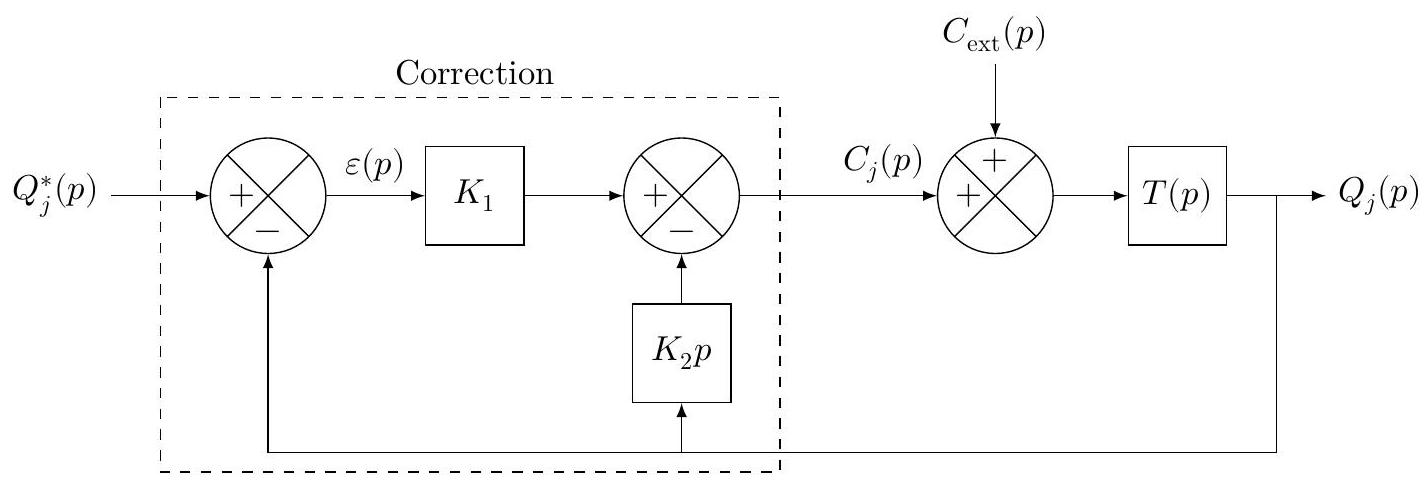
\includegraphics[width=.7\textwidth]{2024_08_29_b4f920ed3822451bf72bg-10}
\caption{\label{fig_11}Modèle de synthèse de la chaine d'asservissement d'une articulation}
\end{figure}

Les mesures disponibles étant réalisées au moyen de capteurs placés directement sur les motoréducteurs pour des questions de facilité de réalisation, on suppose que les grandeurs disponibles sont les positions angulaires des articulations. Pour cette raison, l'asservissement des axes est réalisé sur les mesures des positions angulaires des articulations et non directement sur les positions cartésiennes. Le cahier des charges partiel de cet asservissement est donné par le diagramme des exigences de la figure \ref{fig_12} déduit des exigences exprimées dans le repère cartésien du cahier des charges figure \ref{fig_03}.

\begin{figure}[!h]
\centering
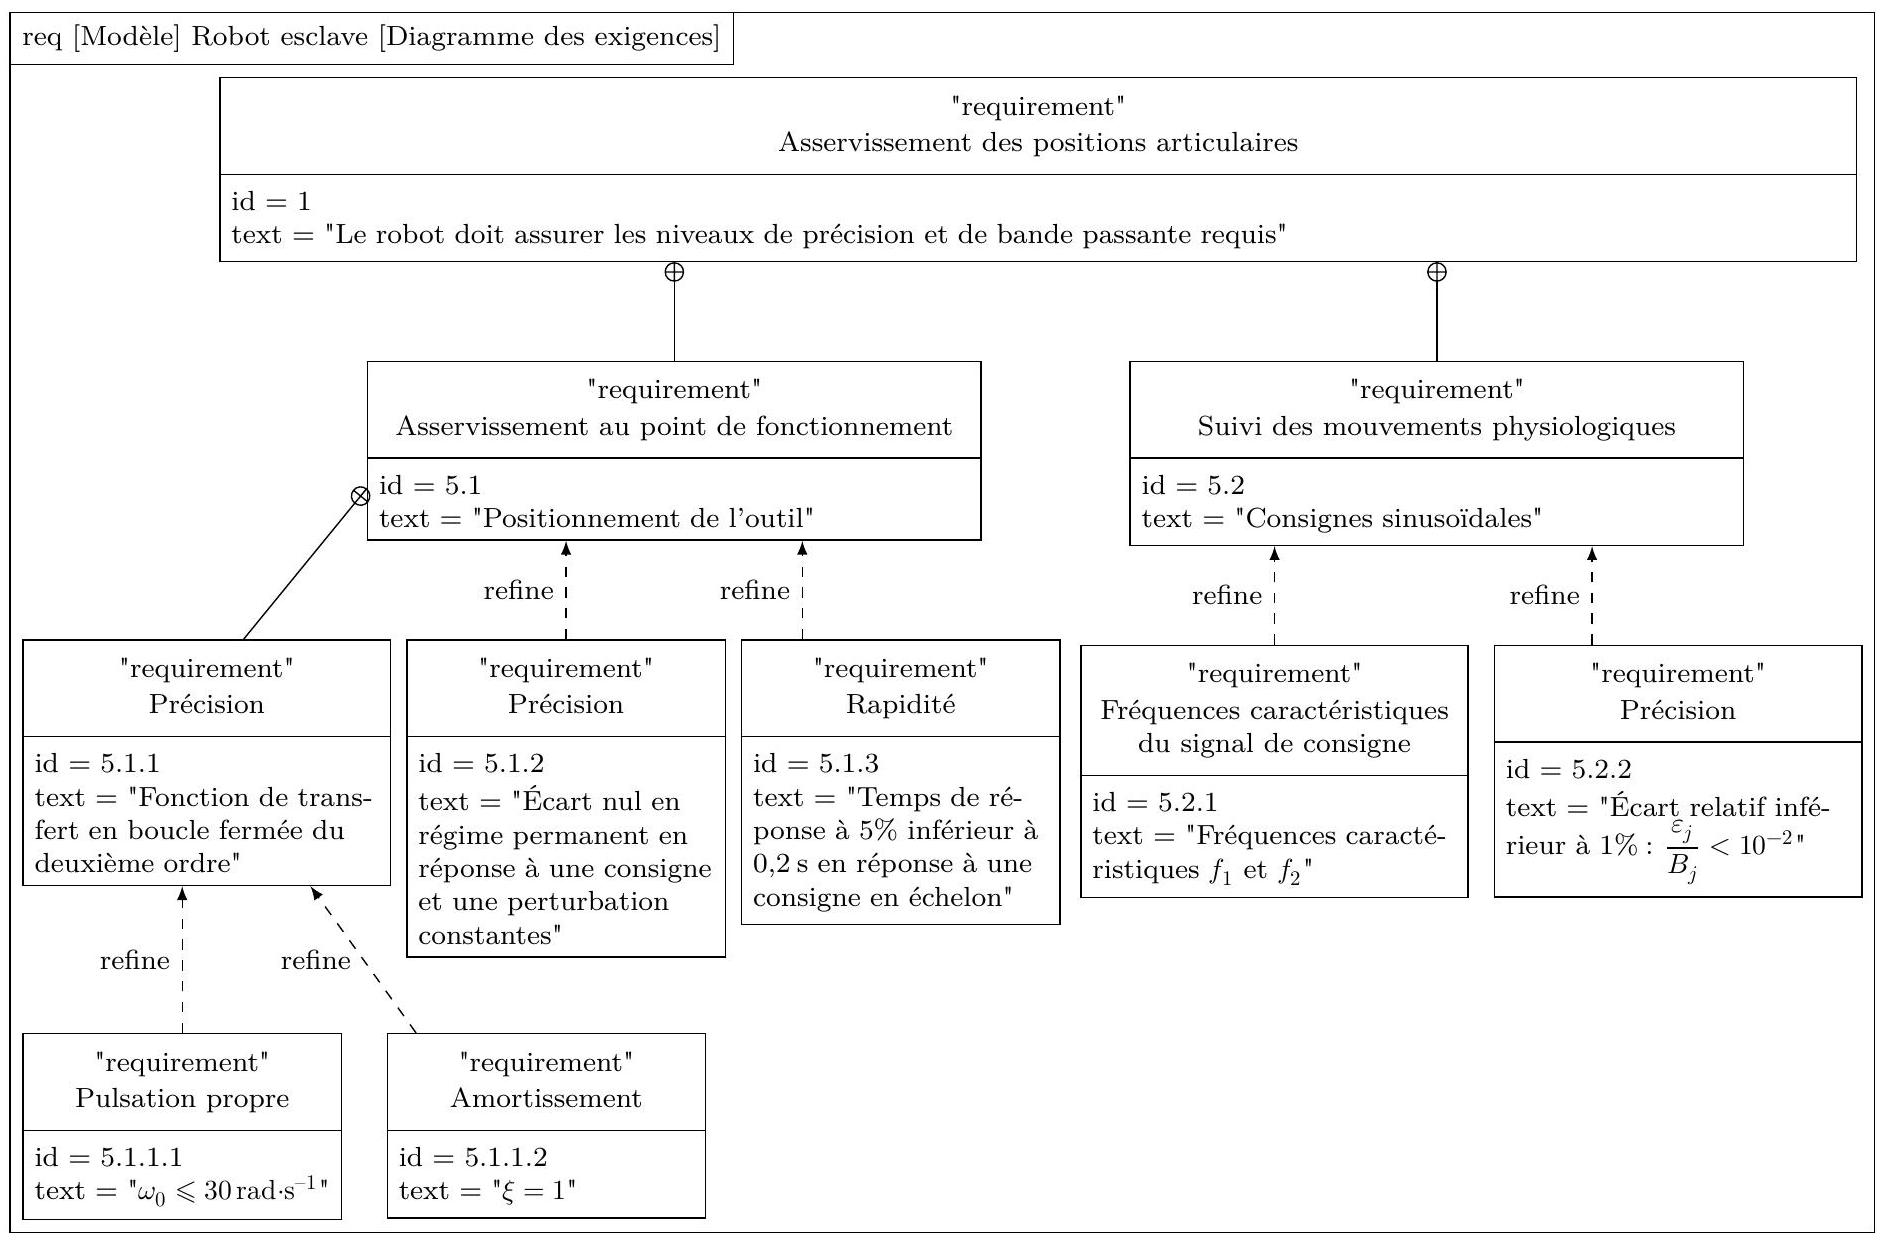
\includegraphics[max width=\textwidth]{2024_08_29_b4f920ed3822451bf72bg-11}
\caption{\label{fig_12}Diagramme des exigences de la chaine d'asservissement}
\end{figure}

%Q 24. 
\question{Déterminer l'expression de $T(p)$. Exprimer, sous forme canonique, la fonction de transfert en boucle fermée $F_{j}(p)=\frac{Q_{j}(p)}{Q_{j}^{*}(p)}$ en fonction de $J_{e q}, K_{1}$ et $K_{2}$. Déterminer alors les expressions littérales de $K_{1}$ et $K_{2}$ en fonction de $J_{e q}$, de la pulsation propre $\omega_{0}$ et de l'amortissement $\xi$ (exigence 5.1.1 du cahier des charges figure \ref{fig_12}).}

Un des problèmes majeurs de ce type de robot, surtout aux faibles vitesses de déplacement, est la présence d'efforts de frottement sec de valeur importante qui peuvent se traduire par des oscillations aux faibles vitesses ou encore par des erreurs en régime permanent. Pour l'analyse en régime permanent, une solution est de modéliser ce type d'effort comme un signal perturbateur externe constant.\\

%Q 25. 
\question{En conservant les gains $K_{1}$ et $K_{2}$ déterminés précédemment, préciser la fonction de transfert en boucle fermée $D(p)=\frac{Q_{j}(p)}{C_{\text {ext }}(p)}$ en fonction de $J_{e q}, \omega_{0}$ et $\xi$. Déterminer alors littéralement l'écart en régime permanent, $\lim _{t \rightarrow+\infty} \varepsilon(t)$, pour une variation en échelon de l'effort perturbateur $c_{\text {ext }}(t)=C_{\text {ext } 0} \Upsilon(t)$ d'amplitude $C_{\text {ext } 0}$ où $\Upsilon(t)$ représente l'échelon d'Heaviside. Conclure sur la performance associée.}

%III.B - 
\subsection{Amélioration des performances par compensation du couple de perturbation}
%Objectif\\
\begin{obj}
Améliorer les performances de la loi de commande vis-à-vis des couples perturbateurs extérieurs.
\end{obj}

Une solution pour améliorer la performance en précision serait de compléter le correcteur en introduisant un terme intégral. Cependant, l'introduction de ce terme diminuera les marges de stabilité et son calcul peut s'avérer difficile au regard de la fonction de transfert en boucle ouverte s'il est nécessaire d'assurer un certain niveau de performance dynamique.

Une solution alternative est de compenser le terme perturbateur en introduisant une loi de commande $c_{j}(t)=$ $\tilde{c}_{j}(t)-c_{\text {ext }}(t)$ (soit après compensation, un modèle du procédé à considérer $J_{e q} \ddot{q}_{j}(t)=\tilde{c}_{j}(t)$ ne faisant pas apparaître de terme perturbateur). Cependant, cette solution nécessite de disposer de la mesure du signal perturbateur, irréalisable en pratique. Afin de répondre à ce problème, une solution est de mettre en place un observateur permettant d'obtenir une estimée $\hat{c}_{\text {ext }}(t)$ du couple extérieur. Cet observateur est mis en place en utilisant les relations suivantes

$$
\left\{\begin{array}{l}
\hat{Q}_{j}(p)=T(p)\left(C_{j}(p)+\hat{C}_{\mathrm{ext}}(p)\right) \\
\hat{C}_{\mathrm{ext}}(p)=K(p)\left(Q_{j}(p)-\hat{Q}_{j}(p)\right)
\end{array}\right.
$$

où $K(p)$ est un correcteur à déterminer et $\hat{Q}_{j}(p)$ une estimation de $Q_{j}(p)$.\\

%Q 26. 
\question{En utilisant ces équations, compléter le schéma bloc modélisant cet observateur (figure \ref{fig_B} du document réponse).}

\question{Au moyen d'une approche à choisir, montrer que le schéma bloc de la figure \ref{fig_B} , représentatif de l'observateur, peut être réduit au schéma bloc équivalent de la figure \ref{fig_13}.}

\begin{figure}[!h]
\centering
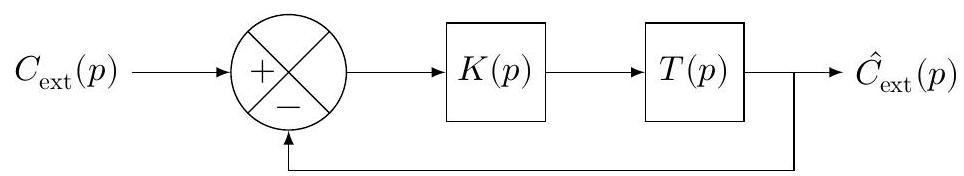
\includegraphics[width=.6\textwidth]{2024_08_29_b4f920ed3822451bf72bg-12}
\caption{\label{fig_13} Modèle équivalent de l'estimateur du couple perturbateur}
\end{figure}


Le calcul du correcteur $K(p)$ peut être alors effectué en utilisant le schéma bloc de la figure \ref{fig_13} où $C_{\text {ext }}(p)$ peut être interprété comme une consigne fictive.

%Q 28. 
\question{En adoptant une démarche comparable à celle utilisée dans la sous-partie III.A, proposer la fonction de transfert d'un correcteur $K(p)$ à deux paramètres, notés $K_{1}^{\prime}$ et $K_{2}^{\prime}$, de façon à ce que la fonction de transfert en boucle fermée ait un polynôme caractéristique du second ordre $\left(p+\omega_{0}^{\prime}\right)^{2}$, d'amortissement $\xi=1$ et de pulsation propre $\omega_{0}^{\prime}=5 \omega_{0}$. Exprimer littéralement ces deux paramètres en fonction de $J_{e q}, \omega_{0}$ et $\xi$. On s'attachera à justifier brièvement que l'erreur en régime permanent est nulle vis-à-vis d'un couple $c_{\text {ext }}$ constant, c'est à dire que $\lim _{t \rightarrow \infty}\left(c_{\text {ext }}(t)-\hat{c}_{\text {ext }}(t)\right)=0$ en réponse à une variation en échelon du couple perturbateur $c_{\text {ext }}(t)=C_{\text {ext } 0} \Upsilon(t)$.}

Cette première structure de commande correspondant à la relation

$$
C_{j}(p)=\tilde{C}_{j}(p)-\hat{C}_{\text {ext }}(p)=\left(K_{1}\left(Q_{j}^{*}(p)-Q_{j}(p)\right)-K_{2} p Q_{j}(p)\right)-\hat{C}_{\text {ext }}(p)
$$

peut être représentée par le schéma bloc de la figure \ref{fig_14}. Elle sera conservée et complétée dans la suite de l'étude.


\begin{figure}[!h]
\centering
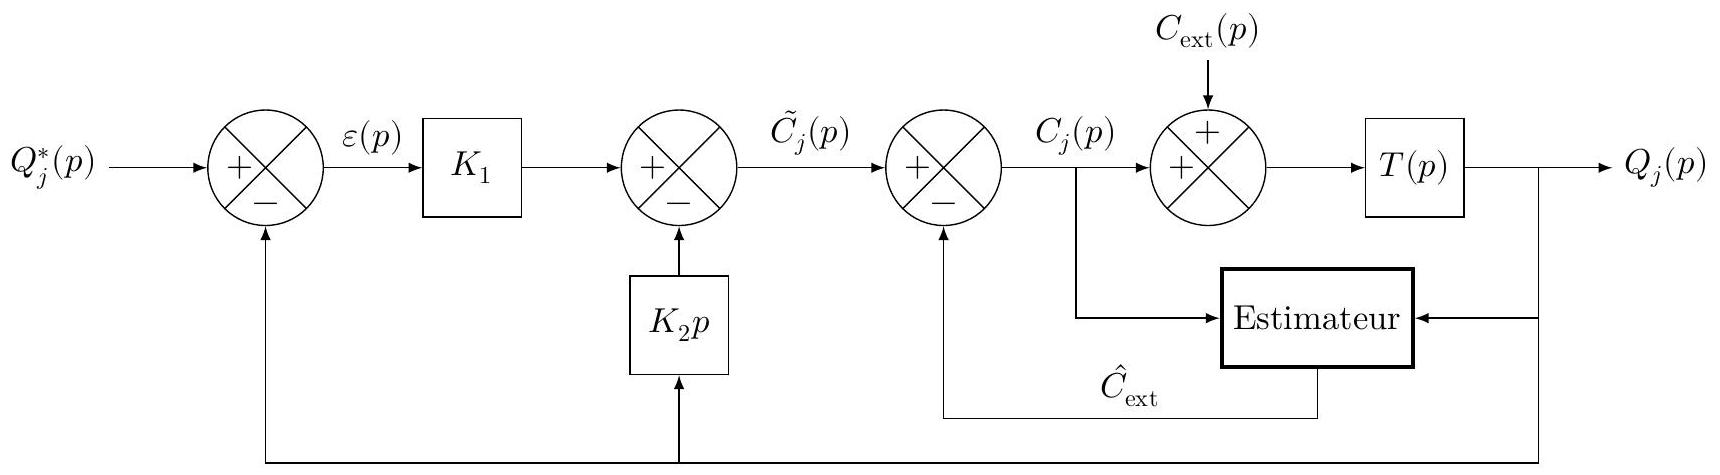
\includegraphics[width=.9\textwidth]{2024_08_29_b4f920ed3822451bf72bg-12(1)}
\caption{\label{fig_14} Schéma bloc de la commande avec estimation et compensation de couple perturbateur}
\end{figure}


L'introduction de la compensation $C_{j}(p)=\left(K_{1}\left(Q_{j}^{*}(p)-Q_{j}(p)\right)-K_{2} p Q_{j}(p)\right)-\hat{C}_{\text {ext }}(p)$ de la perturbation modifie la structure de la boucle et la stabilité en boucle fermée n'est plus garantie à priori.

%Q 29. 
\question{En utilisant cette compensation, déterminer la fonction de transfert $\frac{Q_{j}(p)}{C_{\text {ext }}}$ et l'exprimer en fonction de $T(p), K_{1}, K_{2}$ et $K(p)$ (on supposera que la consigne est nulle $Q_{j}^{*}=0$ et que le système est bouclé par le correcteur déterminé à la sous-partie III.A). En déduire le polynôme caractéristique puis, en justifiant la réponse, conclure sur la stabilité du système bouclé et sur l'écart en régime permanent lorsque le couple perturbateur $c_{\text {ext }}$ est constant.}

\section{Analyse des performances vis-à-vis des mouvements respiratoires}
\begin{obj}
Quantifier le niveau de performance de la loi de commande déterminée en considérant la consigne correspondant aux mouvements physiologiques. Une amélioration de la loi de commande est ensuite envisagée sous la forme d'une anticipation sur la consigne pour améliorer les performances.
\end{obj}

Cette partie porte sur l'analyse et l'amélioration des performances vis-à-vis des signaux respiratoires. Pour ce type de signaux, la consigne de position angulaire est modélisée par le signal $q_{j}^{*}(t)=B \sin (\omega t)$ où l'amplitude $B$ (comprise entre 0,04 et $\SI{0,09}{rad}$ ) et la pulsation $\omega$ (comprise entre les deux valeurs $\omega_{1}$ et $\omega_{2}$ ) sont calculées à partir des deux termes sinusoïdaux retenus dans la partie I.A. On considère le schéma de la figure \ref{fig_11}, on suppose que la structure de correction permet d'assurer la pulsation propre $\omega_{0}$ souhaitée en boucle fermée et que les perturbations extérieures sont nulles $\left(C_{\text {ext }}=0\right)$.\\

%Q 30. 
\question{La fonction de transfert de la consigne $Q_{j}^{*}(p)$ vers l'écart $\varepsilon(p)$, obtenue à partir du schéma bloc de la figure \ref{fig_11}, peut être approchée dans la bande de pulsations $\omega \ll \omega_{0}$, caractéristique des signaux de consigne, par la relation $\frac{\varepsilon(p)}{Q_{j}^{*}(p)} \approx 0,066 p$. En utilisant cette approximation, calculer l'amplitude de l'écart en régime permanent vis-à-vis des deux termes de consigne sinusoïdaux retenus pour modéliser les mouvements respiratoires. Conclure sur cette performance comparativement aux exigences de précision du cahier des charges exprimées dans la figure \ref{fig_12}.}

Afin d'améliorer ce niveau de performance, on complète la loi de commande en ajoutant un terme d'anticipation $c_{a}(t)$ selon la structure de commande représentée d'un point de vue symbolique par le schéma de la figure \ref{fig_15} (pour cette partie, on ne tiendra pas compte des perturbations, seule la structure représentée sur ce schéma bloc sera considérée). La conception de ce terme d'anticipation est l'objectif de la suite de l'étude.

\begin{figure}[!h]
\centering
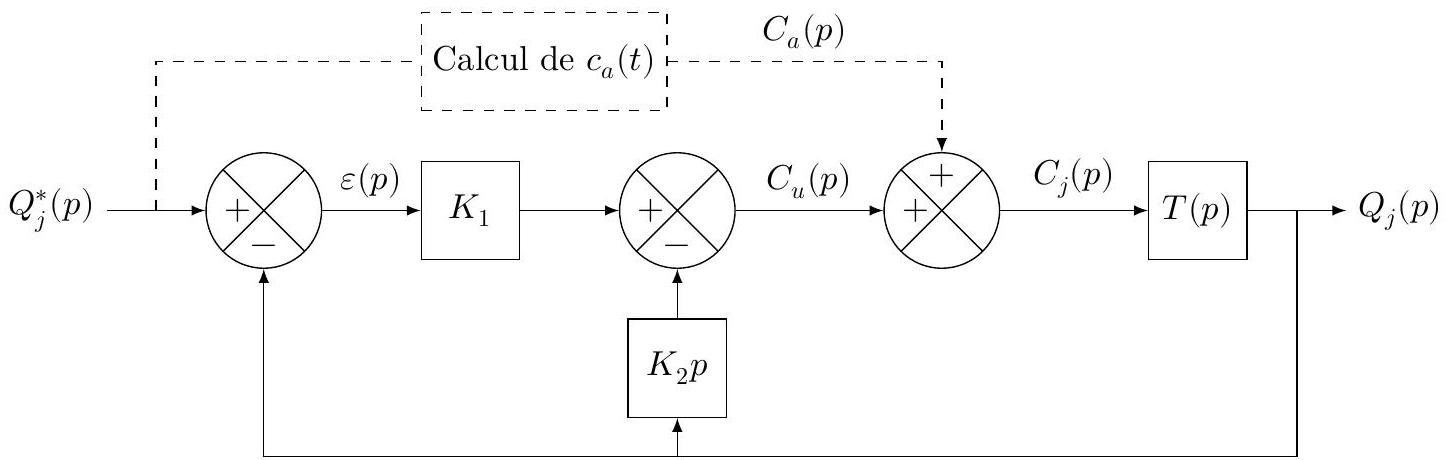
\includegraphics[width=.9\textwidth]{2024_08_29_b4f920ed3822451bf72bg-13}
\caption{\label{fig_15} Structure de commande avec anticipation sur la consigne}
\end{figure}

%Q 31. 
\question{En utilisant les différents éléments de la structure représentée, en particulier la fonction de transfert $T(p)=\frac{Q_{j}(p)}{C_{j}(p)}$, et en supposant que la consigne est idéalement suivie sans erreur, c'est à dire $q_{j}(t) \equiv q_{j}^{*}(t)$, donner en fonction de $q_{j}^{*}(t)$ et de ses dérivées l'expression temporelle du couple idéal $c_{j}(t)$ et du couple $c_{u}(t)$ issu du correcteur. En déduire alors l'expression du terme d'anticipation $c_{a}(t)$ qu'il est nécessaire d'ajouter pour obtenir le comportement souhaité.}

La structure de commande avec anticipation sur la consigne peut être réalisée selon le schéma bloc de la figure \ref{fig_16}.

\begin{figure}[!h]
\centering
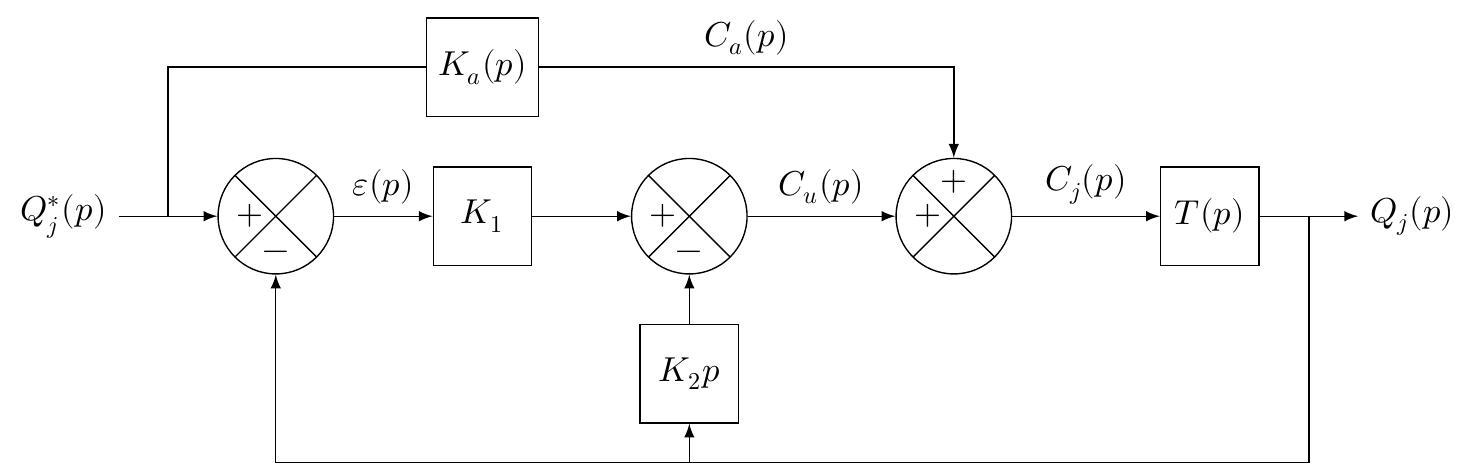
\includegraphics[width=.9\textwidth]{2024_08_29_b4f920ed3822451bf72bg-13(1)}
\caption{\label{fig_16} Structure de commande avec anticipation sur consigne}
\end{figure}


%Q 32. 
\question{Au regard de cette représentation (figure \ref{fig_16}):}
\textit{\begin{itemize}
  \item déterminer la fonction de transfert du correcteur par anticipation $K_{a}(p)$;
  \item déterminer la fonction de transfert en boucle fermée $F(p)=\frac{Q_{j}(p)}{Q_{j}^{*}(p}$. Justifier alors que l'erreur est nulle vis-à-vis de la consigne et en particulier vis-à-vis de signaux de consigne sinusoïdaux.\\
\end{itemize}}

Une fonction telle que $K_{a}(p)$ est difficile à réaliser en pratique, voire impossible. La réalisation de la loi de commande est numérique et on implante cette loi de commande selon la structure de la figure \ref{fig_17} en séparant le mouvement périodique dû à la respiration $\delta q_{j}^{*}(t)=B_{1} \sin \left(\omega_{1} t+\theta_{1}\right)+B_{2} \sin \left(\omega_{2} t+\theta_{2}\right)$ de la partie due à la consigne correspondant au point de fonctionnement $Q_{j 0}^{*}(p)$.


\begin{figure}[!h]
\centering
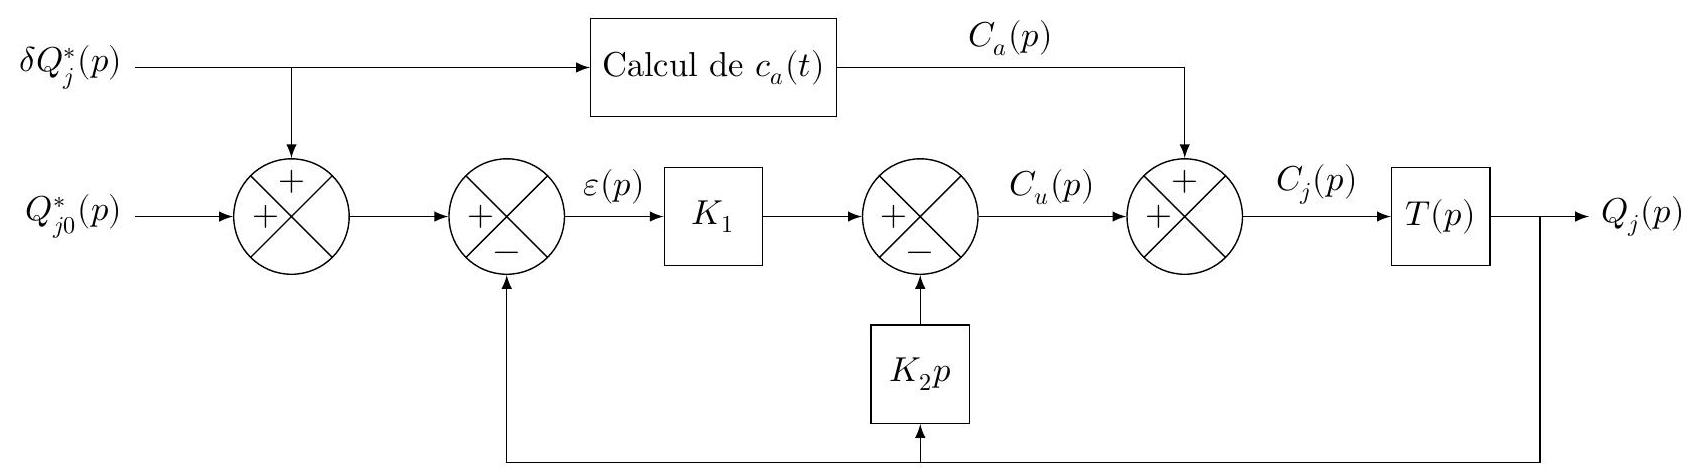
\includegraphics[max width=\textwidth]{2024_08_29_b4f920ed3822451bf72bg-14}
\caption{\label{fig_17} Schéma d'implantation de la structure de commande avec anticipation sur la consigne}
\end{figure}

%Q 33. 
\question{Donner alors l'équation permettant de calculer le signal d'anticipation $c_{a}(t)$ pour le cas du signal $\delta q_{j}^{*}(t)$ sinusoïdal retenu pour modéliser les mouvements physiologiques.}

\paragraph*{Question de synthèse}

En adoptant cette stratégie de commande :
\begin{itemize}
  \item la figure \ref{fig_18} montre le déplacement de la position angulaire de l'axe 3 en réponse à une variation en échelon d'amplitude $\SI{0,3}{rad}$ de la consigne ;
  \item la figure \ref{fig_19} montre les évolutions de la consigne sinusoïdale destinée à suivre les mouvements physiologiques, de la sortie et du signal d'écart associé.
\end{itemize}

\begin{figure}[!h]
\centering
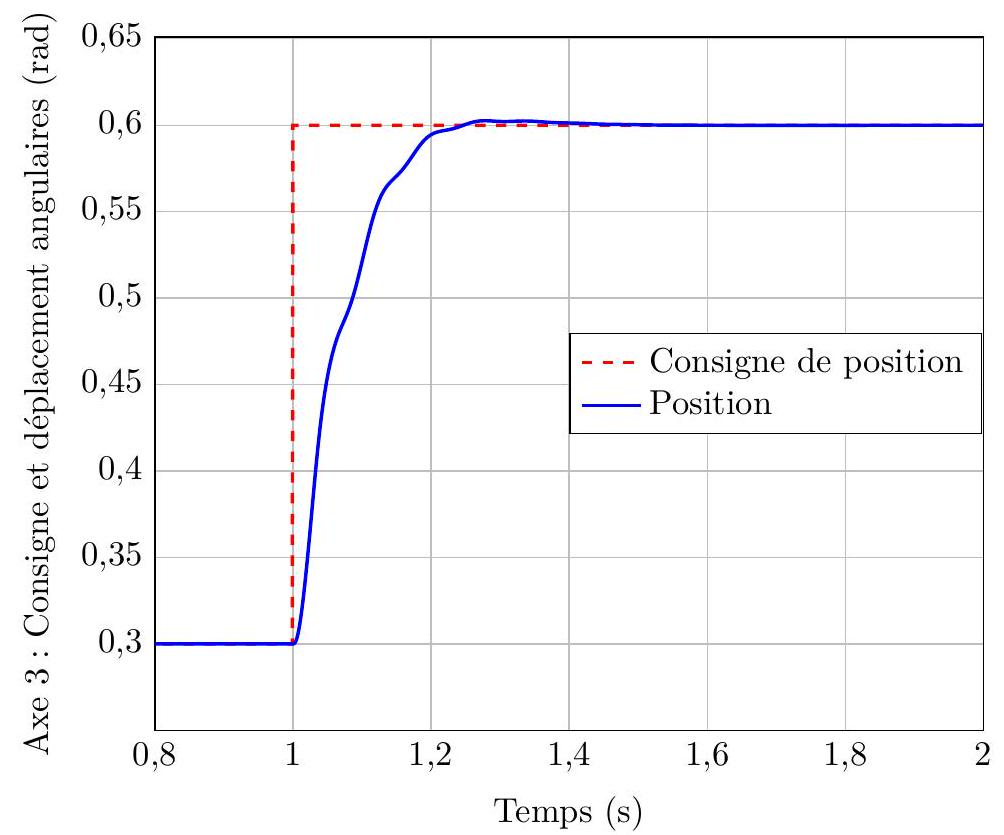
\includegraphics[max width=.7\textwidth]{2024_08_29_b4f920ed3822451bf72bg-14(1)}

\caption{\label{fig_18} Axe 3 : réponse à une variation en échelon d'amplitude $0,3 \mathrm{rad}$ de la consigne de position articulaire}
\end{figure}

%Q 34. 
\question{Analyser les réponses obtenues et conclure (en argumentant la réponse) sur la pertinence de ce système au regard de la problématique de compensation des mouvements physiologiques pour les robots de téléopération en chirurgie mini-invasive.}

